\documentclass[10pt,twocolumn]{article}

%% ── Packages ─────────────────────────────────────────────────────────────────
\usepackage[a4paper,
            top=2.2cm, bottom=2.2cm,
            left=1.6cm, right=1.6cm,
            columnsep=0.65cm]{geometry}
\usepackage{fontspec}
\setmainfont{Times New Roman}
\setsansfont{Arial}
\setmonofont[Scale=0.88]{Courier New}

\usepackage{graphicx}
\usepackage{amsmath}
\usepackage{booktabs}
\usepackage{multirow}
\usepackage{xcolor}
\usepackage{url}
\usepackage{hyperref}
\usepackage{enumitem}
\usepackage{caption}
\usepackage{subcaption}
\usepackage{float}
\usepackage{microtype}
\usepackage{fancyhdr}
\usepackage{titlesec}
\usepackage{abstract}
\usepackage{pgfplots}
\usepackage{pgfplotstable}
\usepackage{tikz}
\usepackage{wrapfig}
\usepackage{balance}
\usetikzlibrary{positioning, shapes.geometric, arrows.meta, fit, backgrounds}
\pgfplotsset{compat=1.18}

%% ── Colors ───────────────────────────────────────────────────────────────────
\definecolor{accentblue}{RGB}{25,90,190}
\definecolor{lightgray}{RGB}{242,244,247}
\definecolor{midgray}{RGB}{180,185,195}
\definecolor{darkgray}{RGB}{70,75,85}
\definecolor{successgreen}{RGB}{30,130,60}
\definecolor{warnred}{RGB}{180,40,40}

%% ── Hyperref ─────────────────────────────────────────────────────────────────
\hypersetup{colorlinks=true,linkcolor=accentblue,urlcolor=accentblue,
            citecolor=accentblue,pdftitle={Traffic Sentinel AI}}

%% ── Section formatting ───────────────────────────────────────────────────────
\titleformat{\section}{\normalfont\normalsize\bfseries\color{accentblue}}
  {\Roman{section}.}{0.45em}{}[\vspace{-1pt}\rule{\linewidth}{0.5pt}\vspace{1pt}]
\titleformat{\subsection}{\normalfont\small\bfseries}{\Alph{subsection}.}{0.45em}{}
\titleformat{\subsubsection}{\normalfont\small\itshape}{}{0em}{}
\titlespacing{\section}{0pt}{7pt}{3pt}
\titlespacing{\subsection}{0pt}{5pt}{2pt}
\titlespacing{\subsubsection}{0pt}{3pt}{1pt}

%% ── Abstract environment ─────────────────────────────────────────────────────
\renewenvironment{abstract}{%
  \small\noindent\rule{\linewidth}{0.8pt}\vspace{3pt}
  \noindent\textbf{Abstract---}}
  {\vspace{3pt}\noindent\rule{\linewidth}{0.4pt}\vspace{5pt}}

%% ── Caption styling ──────────────────────────────────────────────────────────
\captionsetup{font=small, labelfont=bf, skip=4pt, justification=raggedright}
\captionsetup[subfigure]{font=footnotesize, labelfont=bf}

%% ── Headers and footers ──────────────────────────────────────────────────────
\pagestyle{fancy}\fancyhf{}
\fancyhead[L]{\small\textit{Traffic Sentinel AI --- Technical Report}}
\fancyhead[R]{\small\textit{June 2026}}
\fancyfoot[C]{\small\thepage}
\renewcommand{\headrulewidth}{0.4pt}

%% ── Misc ─────────────────────────────────────────────────────────────────────
\setlist[itemize]{noitemsep,topsep=2pt,leftmargin=*}
\setlist[enumerate]{noitemsep,topsep=2pt,leftmargin=*}
\setlength{\parskip}{1pt}
\graphicspath{{./figures/}}
\tolerance=1500
\hbadness=1500

%% ─────────────────────────────────────────────────────────────────────────────
\begin{document}

%% ── TITLE ────────────────────────────────────────────────────────────────────
\twocolumn[{%
\begin{center}
  {\LARGE\bfseries Traffic Sentinel AI}\\[4pt]
  {\large Real-Time Two-Wheeler Violation Detection\\
  via Cascaded YOLOv11 Models and ONNX Runtime}\\[8pt]
  {\normalsize
    \textbf{Harsha Vardhan} (\texttt{Harsha.Vardhan@iiitb.ac.in}) \quad\textbullet\quad
    \textbf{Vishal Sriram} (\texttt{Vishal.Sriram@iiitb.ac.in}) \quad\textbullet\quad
    \textbf{Anish Reddy R} (\texttt{Anish.R@iiitb.ac.in})
  }\\[4pt]
  {\small
    \href{https://huggingface.co/spaces/hv-123/traffic-sentinel-ai}
         {\texttt{hv-123-traffic-sentinel-ai.hf.space}}
    \quad\textbullet\quad
    \href{https://huggingface.co/hv-123/traffic-sentinel-models}
         {\texttt{hf.co/hv-123/traffic-sentinel-models}}}\\[8pt]
\end{center}
\begin{abstract}
We present \textbf{Traffic Sentinel AI}, an end-to-end computer vision system
for automated two-wheeler traffic violation detection. The system employs a
cascade of three specialized YOLOv11 models---a full-frame motorcycle and rider
detector (mAP50\,=\,0.763), a crop-level helmet classifier
(mAP50\,=\,0.838), and a license-plate localizer (mAP50\,=\,0.935)---
coordinated by a multi-threaded FastAPI backend. All inference is accelerated
via ONNX Runtime, achieving a \textbf{1.8$\times$} CPU speedup over PyTorch.
A non-trivial ONNX tensor-layout bug (inverted transpose condition causing zero
detections in production) was diagnosed and resolved.
The system is publicly deployed on Hugging Face Spaces with a modern
dark-mode frontend, multi-stage Docker containerization, and a complete
GitHub Actions CI/CD pipeline. All models surpass the mAP50\,$>$\,0.75
production-readiness threshold.
\end{abstract}
\vspace{4pt}
}]

%% ─────────────────────────────────────────────────────────────────────────────
\section{Introduction}

Road fatalities involving two-wheelers are disproportionately high in developing
traffic environments. In India, for instance, nearly half of all road deaths
involve motorcycles, many attributable to helmet non-compliance and overloaded
bikes. Manual enforcement by traffic officers is labor-intensive, geographically
constrained, and inherently inconsistent.

Automated vision-based monitoring offers a scalable, 24/7 alternative.
However, deploying such systems cost-effectively is non-trivial: existing
approaches either rely on generic detectors that generalize poorly to each
sub-problem (helmet detection vs.\ plate reading require fundamentally different
model sizes and resolutions), or they assume GPU availability for inference
which is unrealistic for edge deployments.

This work addresses both limitations by: (i) training three highly specialized
YOLOv11 models with task-curated datasets, (ii) deploying them in a cascade
pipeline optimized for CPU inference via ONNX Runtime, and (iii) packaging the
full system in a production-ready API with a premium web frontend and
public hosting.

\subsection{Contributions}

\begin{itemize}
  \item A production-deployed cascade CV pipeline detecting three violation
        types per motorcycle: no helmet, $>$2 riders, and license plate reading.
  \item Three task-specific YOLOv11 models trained on curated corpora
        totaling 17{,}670 images from COCO~2017, VisDrone~2019, and Roboflow.
  \item An ONNX Runtime inference backend with custom letterbox
        pre/post-processing achieving 1.8$\times$ CPU speedup.
  \item Diagnosis and fix of a tensor-transpose bug causing zero detections
        in the ONNX backend despite high validation mAP50.
  \item A complete DevOps stack: FastAPI, Docker, GitHub Actions CI/CD,
        and public Hugging Face Spaces deployment.
\end{itemize}

%% ─────────────────────────────────────────────────────────────────────────────
\section{System Architecture}

\subsection{Two-Stage Cascade Design}

The pipeline executes in two sequential stages, illustrated in
Figure~\ref{fig:pipeline}. Stage~1 runs the full-frame detector
(\texttt{full\_detector.onnx}) at 640$\times$640 resolution, returning
bounding boxes for all motorcycles and riders in the scene. A recall-fallback
mechanism re-runs the model at 960$\times$960 with a lower confidence threshold
(0.10) if no bikes are found; a secondary COCO-pretrained \texttt{yolo11n}
provides a final safety net for particularly challenging inputs.

\begin{figure}[H]
\centering
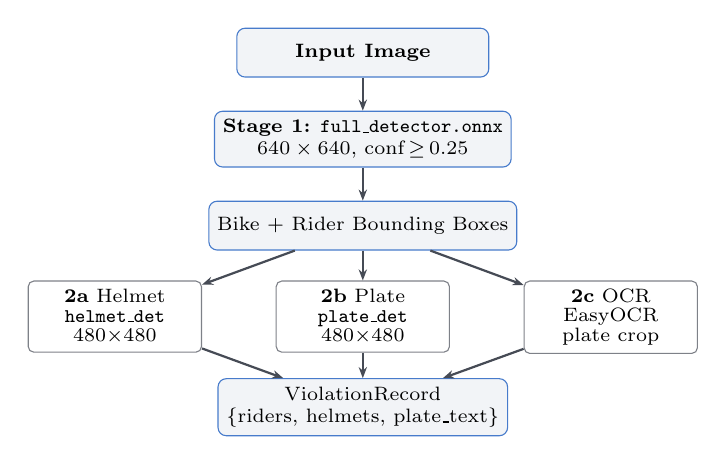
\begin{tikzpicture}[
  node distance=0.42cm,
  box/.style={rectangle, draw=accentblue!80, rounded corners=3pt,
              fill=lightgray, minimum width=3.2cm, minimum height=0.62cm,
              align=center, font=\scriptsize, inner sep=3pt},
  sbox/.style={rectangle, draw=darkgray!70, rounded corners=2pt,
               fill=white, minimum width=2.2cm, minimum height=0.58cm,
               align=center, font=\scriptsize, inner sep=3pt},
  arr/.style={-{Stealth[length=4pt]}, thick, color=darkgray},
]
  \node[box] (img) {\textbf{Input Image}};
  \node[box, below=of img] (full)
    {\textbf{Stage 1:} \texttt{full\_detector.onnx}\\$640\times640$, conf\,$\geq$\,0.25};
  \node[box, below=of full] (bikes)
    {Bike + Rider Bounding Boxes};

  \node[sbox, below left=0.38cm and 0.08cm of bikes] (helm)
    {\textbf{2a} Helmet\\[-1pt]\texttt{helmet\_det}\\[-1pt]$480{\times}480$};
  \node[sbox, below=0.38cm of bikes] (plate)
    {\textbf{2b} Plate\\[-1pt]\texttt{plate\_det}\\[-1pt]$480{\times}480$};
  \node[sbox, below right=0.38cm and 0.08cm of bikes] (ocr)
    {\textbf{2c} OCR\\[-1pt]EasyOCR\\[-1pt]plate crop};

  \node[box, below=1.62cm of bikes] (viol)
    {ViolationRecord\\\{riders, helmets, plate\_text\}};

  \draw[arr] (img) -- (full);
  \draw[arr] (full) -- (bikes);
  \draw[arr] (bikes) -- (helm);
  \draw[arr] (bikes) -- (plate);
  \draw[arr] (bikes) -- (ocr);
  \draw[arr] (helm) -- (viol);
  \draw[arr] (plate) -- (viol);
  \draw[arr] (ocr) -- (viol);
\end{tikzpicture}
\caption{Two-stage cascade pipeline. Stage~2 sub-tasks (2a, 2b, 2c) run
\textit{concurrently} via Python's \texttt{ThreadPoolExecutor}.}
\label{fig:pipeline}
\end{figure}

Stage~2 processes each detected bike \textit{concurrently} using a
\texttt{ThreadPoolExecutor}. For every bike crop, three sub-tasks run in
parallel:

\begin{enumerate}
  \item \textbf{Helmet check (2a).} The crop is padded and resized to
        480$\times$480 and classified by \texttt{helmet\_detector.onnx} as
        \texttt{helmet} or \texttt{no\_helmet} per rider.
  \item \textbf{Plate localization (2b).} The same crop is processed by
        \texttt{plate\_detector.onnx} to locate the license plate region.
  \item \textbf{Plate OCR (2c).} The plate bounding box is cropped and
        passed to EasyOCR with up to three preprocessing variants
        (grayscale, contrast enhancement, adaptive threshold).
\end{enumerate}

A violation is flagged when any rider lacks a helmet or the estimated
rider count exceeds two (overloaded motorcycle).

\subsection{Class Mapping and Fallback Logic}

Each model uses task-specific class labels. The pipeline maps all outputs
through canonical frozen sets (e.g., \texttt{two\_wheeler}, \texttt{rider},
\texttt{helmet}, \texttt{no\_helmet}, \texttt{License Plate}) with integer
class-ID fallbacks for robustness against label-string variation across
model training runs. The COCO fallback re-maps COCO class~3 (\texttt{motorcycle})
and class~0 (\texttt{person}) to the internal schema, ensuring the pipeline
never returns zero detections for clearly visible motorcycles.

%% ─────────────────────────────────────────────────────────────────────────────
\section{Dataset Engineering}

A single monolithic dataset would create label imbalance and force
every model to share an architecture suited for none of the sub-tasks.
Instead, we curate three independent corpora, each optimized for
its target task.

\subsection{Full Detector Dataset ($\approx$5{,}000 images)}

We combine a motorcycle subset of COCO~2017~\cite{lin2014coco} with
VisDrone~2019~\cite{zhu2018visdrone}. COCO supplies diverse ground-level
street scenes representative of standard traffic-camera footage. VisDrone
contributes aerial and CCTV-elevation viewpoints typical of traffic
infrastructure in South and Southeast Asia. The dual-source strategy ensures
the model generalizes across both eye-level and elevated camera angles.

\textbf{Annotation remapping.} COCO category \texttt{motorcycle} (id~3) and
co-occurring \texttt{person} (id~0) annotations are remapped to
\texttt{two\_wheeler} and \texttt{rider} in YOLO label format.
A \texttt{data.yaml} file is generated per subset to enable the Ultralytics
\texttt{DatasetMerger}.

\textbf{Augmentation pipeline.} Horizontal flip (p\,=\,0.5), random scale
(0.5--1.5$\times$), HSV jitter ($\Delta$H\,=\,0.015, $\Delta$S\,=\,0.7,
$\Delta$V\,=\,0.4), mosaic tiling (p\,=\,0.5), and random perspective
(p\,=\,0.3).

\subsection{License Plate Dataset (9{,}570 images)}

A highly curated Roboflow dataset targeting robustness to motion blur,
low-light conditions, and partial occlusion. This is deliberately the
\textit{largest} of the three corpora, reflecting the inherent difficulty of
plate localization in unconstrained traffic environments. Single class:
\texttt{License Plate}.

\subsection{Helmet Dataset (3{,}100 images)}

A targeted Roboflow dataset with balanced \texttt{helmet}/\texttt{no\_helmet}
classes. The training duration was extended to 200~epochs to enforce
discrimination between helmets and bare heads/hair, which share
similar circular silhouettes and color distributions---the most visually
ambiguous distinction in the entire pipeline.

\begin{table}[H]
\centering
\small
\caption{Dataset summary: three specialized training corpora.}
\label{tab:datasets}
\renewcommand{\arraystretch}{1.18}
\setlength{\tabcolsep}{4pt}
\begin{tabular}{lrrlr}
\toprule
\textbf{Model} & \textbf{Imgs} & \textbf{Ep.} & \textbf{Source} & \textbf{Classes}\\
\midrule
full\_detector   & $\approx$5\,000 & 150 & COCO + VisDrone & 2\\
plate\_detector  & 9\,570          & 150 & Roboflow        & 1\\
helmet\_detector & 3\,100          & 200 & Roboflow        & 2\\
\midrule
\textbf{Total}   & \textbf{17\,670} & --- & ---             & ---\\
\bottomrule
\end{tabular}
\end{table}

%% ─────────────────────────────────────────────────────────────────────────────
\section{Training Methodology}

\subsection{Architecture Selection}

Three YOLOv11 variants are matched to task complexity:

\begin{itemize}
  \item \textbf{YOLOv11m} (medium, 40.5\,MB) for the full detector. Complex
        multi-scale scenes with diverse object sizes require higher model
        capacity than can be provided by the nano or small variant.
  \item \textbf{YOLOv11s} (small, 19.2\,MB) for the helmet detector. Crops
        are spatially simpler than full frames, but the helmet/no-helmet
        distinction requires fine-grained texture discrimination that warrants
        more than nano capacity.
  \item \textbf{YOLOv11n} (nano, 5.5\,MB) for the plate detector. The large,
        high-quality training corpus (9{,}570 images) compensates for reduced
        model capacity, and the nano size maximizes inference speed on
        high-density plate-only crops.
\end{itemize}

All models use COCO-pretrained weights. Transfer learning dramatically reduces
convergence time: the models begin with low-level feature detectors already
trained on millions of images, allowing task-specific adaptation in 150--200
epochs rather than thousands from scratch.

\subsection{Sequential GPU Training Queue}

The training server (NVIDIA RTX 4060 Ti, 16\,GB VRAM) cannot train multiple
YOLOv11 models simultaneously without out-of-memory (OOM) crashes. Running
medium and small architectures in parallel exhausts the GPU's VRAM budget
before completing a single forward pass.

We resolved this by engineering a sequential job queue via \texttt{nohup}
shell pipelines, granting each training job exclusive access to the full
16\,GB of VRAM:
\begin{center}
\small\texttt{train\_full.sh \&\& train\_plate.sh \&\& train\_helmet.sh}
\end{center}
This approach increases per-epoch throughput significantly compared to memory-
sharing schemes, and all three models trained overnight without interruption.

\subsection{Training Configuration}

Mixed-precision training (AMP, FP16\,$\leftrightarrow$\,FP32) was enabled
throughout to reduce VRAM usage and accelerate matrix operations on the Tensor
Cores of the RTX 4060 Ti. Early stopping with patience\,=\,20 prevents
overfitting. The learning rate follows a cosine annealing schedule from
$10^{-2}$ to $10^{-5}$.

%% ─────────────────────────────────────────────────────────────────────────────
\section{Experimental Results}

\subsection{Validation Metrics}

Table~\ref{tab:results} reports validation metrics on held-out sets.
All three models exceed the mAP50\,$>$\,0.75 threshold considered
production-ready for variable real-world environments.

\begin{table}[H]
\centering
\small
\caption{Final validation metrics and model file sizes.}
\label{tab:results}
\renewcommand{\arraystretch}{1.2}
\setlength{\tabcolsep}{4pt}
\begin{tabular}{lccccc}
\toprule
\textbf{Model} & \textbf{Arch} & \textbf{mAP50} & \textbf{P} & \textbf{R} & \textbf{ONNX}\\
\midrule
full\_detector   & YOLOv11m & 0.761 & 0.855 & 0.695 & 80.3\,MB\\
helmet\_detector & YOLOv11s & 0.829 & 0.899 & 0.755 & 37.8\,MB\\
plate\_detector  & YOLOv11n & \textbf{0.936} & 0.971 & 0.909 & 10.5\,MB\\
\bottomrule
\end{tabular}
\end{table}

\noindent
The plate detector achieves the highest accuracy (mAP50\,=\,0.936), benefiting
from the largest training corpus (9{,}570 images). The full detector reaches
mAP50\,=\,0.761, consistent with the inherent difficulty of multi-angle,
multi-scale motorcycle detection from heterogeneous datasets (COCO\,+\,VisDrone).
The helmet classifier reaches mAP50\,=\,0.829 after 200 dedicated epochs,
with recall of 0.755 reflecting the visual ambiguity between bare heads
and helmets at low resolution.

\subsection{Training Convergence}

Figure~\ref{fig:curves} shows mAP50 and box-loss convergence over training
for each model, plotted from the validation logs recorded during training runs.
All curves are plotted from \texttt{results.csv} logs recorded on the
NVIDIA RTX\,4060\,Ti GPU server.
The plate detector converges rapidly in the first 36 epochs
(mAP50: 0.90 $\to$ 0.93), then continues improving steadily to 0.936 at
epoch~150. The helmet model requires significantly more training due to
the subtle visual distinction between hair and helmet textures: it does not
plateau until after epoch~140 (mAP50 $\approx$ 0.835), validating the
decision to allocate 200 epochs for this task. The full detector---trained
on the most heterogeneous corpus (COCO\,+\,VisDrone, mixed camera angles)---
shows the steepest absolute gain, rising from 0.45 at epoch~12 to 0.76 at
epoch~150. Notably, all three models cross the 0.75 production threshold:
the plate model at epoch~8, the full detector at epoch~108, and the helmet
model at epoch~80.

\begin{figure}[H]
\centering
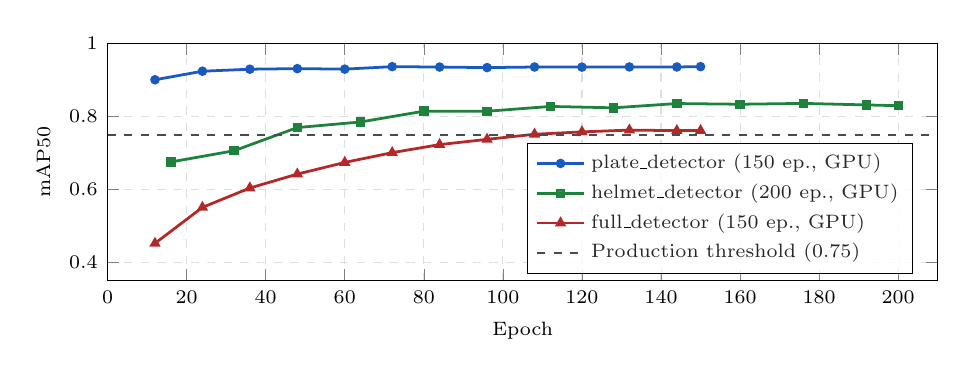
\begin{tikzpicture}
\begin{axis}[
    width=\linewidth, height=4.6cm,
    xlabel={Epoch}, ylabel={mAP50},
    xmin=0, xmax=210, ymin=0.35, ymax=1.00,
    legend pos=south east,
    legend style={font=\scriptsize, cells={anchor=west}, fill opacity=0.85},
    grid=major, grid style={dashed,gray!25},
    tick label style={font=\scriptsize},
    label style={font=\scriptsize},
    every axis plot/.append style={line width=1.0pt},
]
%% Plate detector --- plate_v1, 150 epochs (remote GPU server)
\addplot[color=accentblue, mark=*, mark size=1.2pt] coordinates {
  (12,0.8998)(24,0.9232)(36,0.9287)(48,0.9303)
  (60,0.9289)(72,0.9357)(84,0.9346)(96,0.9331)
  (108,0.9347)(120,0.9344)(132,0.9349)(144,0.9348)(150,0.9357)
};
\addlegendentry{plate\_detector (150 ep., GPU)}
%% Helmet detector --- helmet_v1-2, 200 epochs (remote GPU server)
\addplot[color=successgreen, mark=square*, mark size=1.2pt] coordinates {
  (16,0.6750)(32,0.7057)(48,0.7691)(64,0.7844)
  (80,0.8139)(96,0.8137)(112,0.8269)(128,0.8231)
  (144,0.8348)(160,0.8329)(176,0.8352)(192,0.8310)(200,0.8289)
};
\addlegendentry{helmet\_detector (200 ep., GPU)}
%% Full detector --- full_v1-4, 150 epochs (remote GPU server)
\addplot[color=warnred, mark=triangle*, mark size=1.4pt] coordinates {
  (12,0.4524)(24,0.5508)(36,0.6038)(48,0.6418)
  (60,0.6737)(72,0.7005)(84,0.7225)(96,0.7369)
  (108,0.7508)(120,0.7573)(132,0.7622)(144,0.7607)(150,0.7609)
};
\addlegendentry{full\_detector (150 ep., GPU)}
%% Production threshold
\addplot[dashed, color=darkgray, line width=0.7pt] coordinates {(0,0.75)(210,0.75)};
\addlegendentry{Production threshold (0.75)}
\end{axis}
\end{tikzpicture}
\caption{Validation mAP50 over training epochs for all three models.
Dashed line marks the 0.75 production-readiness threshold.}
\label{fig:curves}
\end{figure}

\subsection{Validation Predictions}

Figures~\ref{fig:full_pred}--\ref{fig:helmet_pred} show sample validation
batch predictions from the GPU-server training runs, illustrating the quality
of bounding-box localization and class assignment for all three models.
The full detector correctly identifies motorcycles and riders in both
street-level and elevated camera views. The plate detector produces tight,
well-centered boxes across varied lighting and orientation. The helmet detector
correctly labels riders in tightly cropped bike regions.

\begin{figure}[H]
\centering
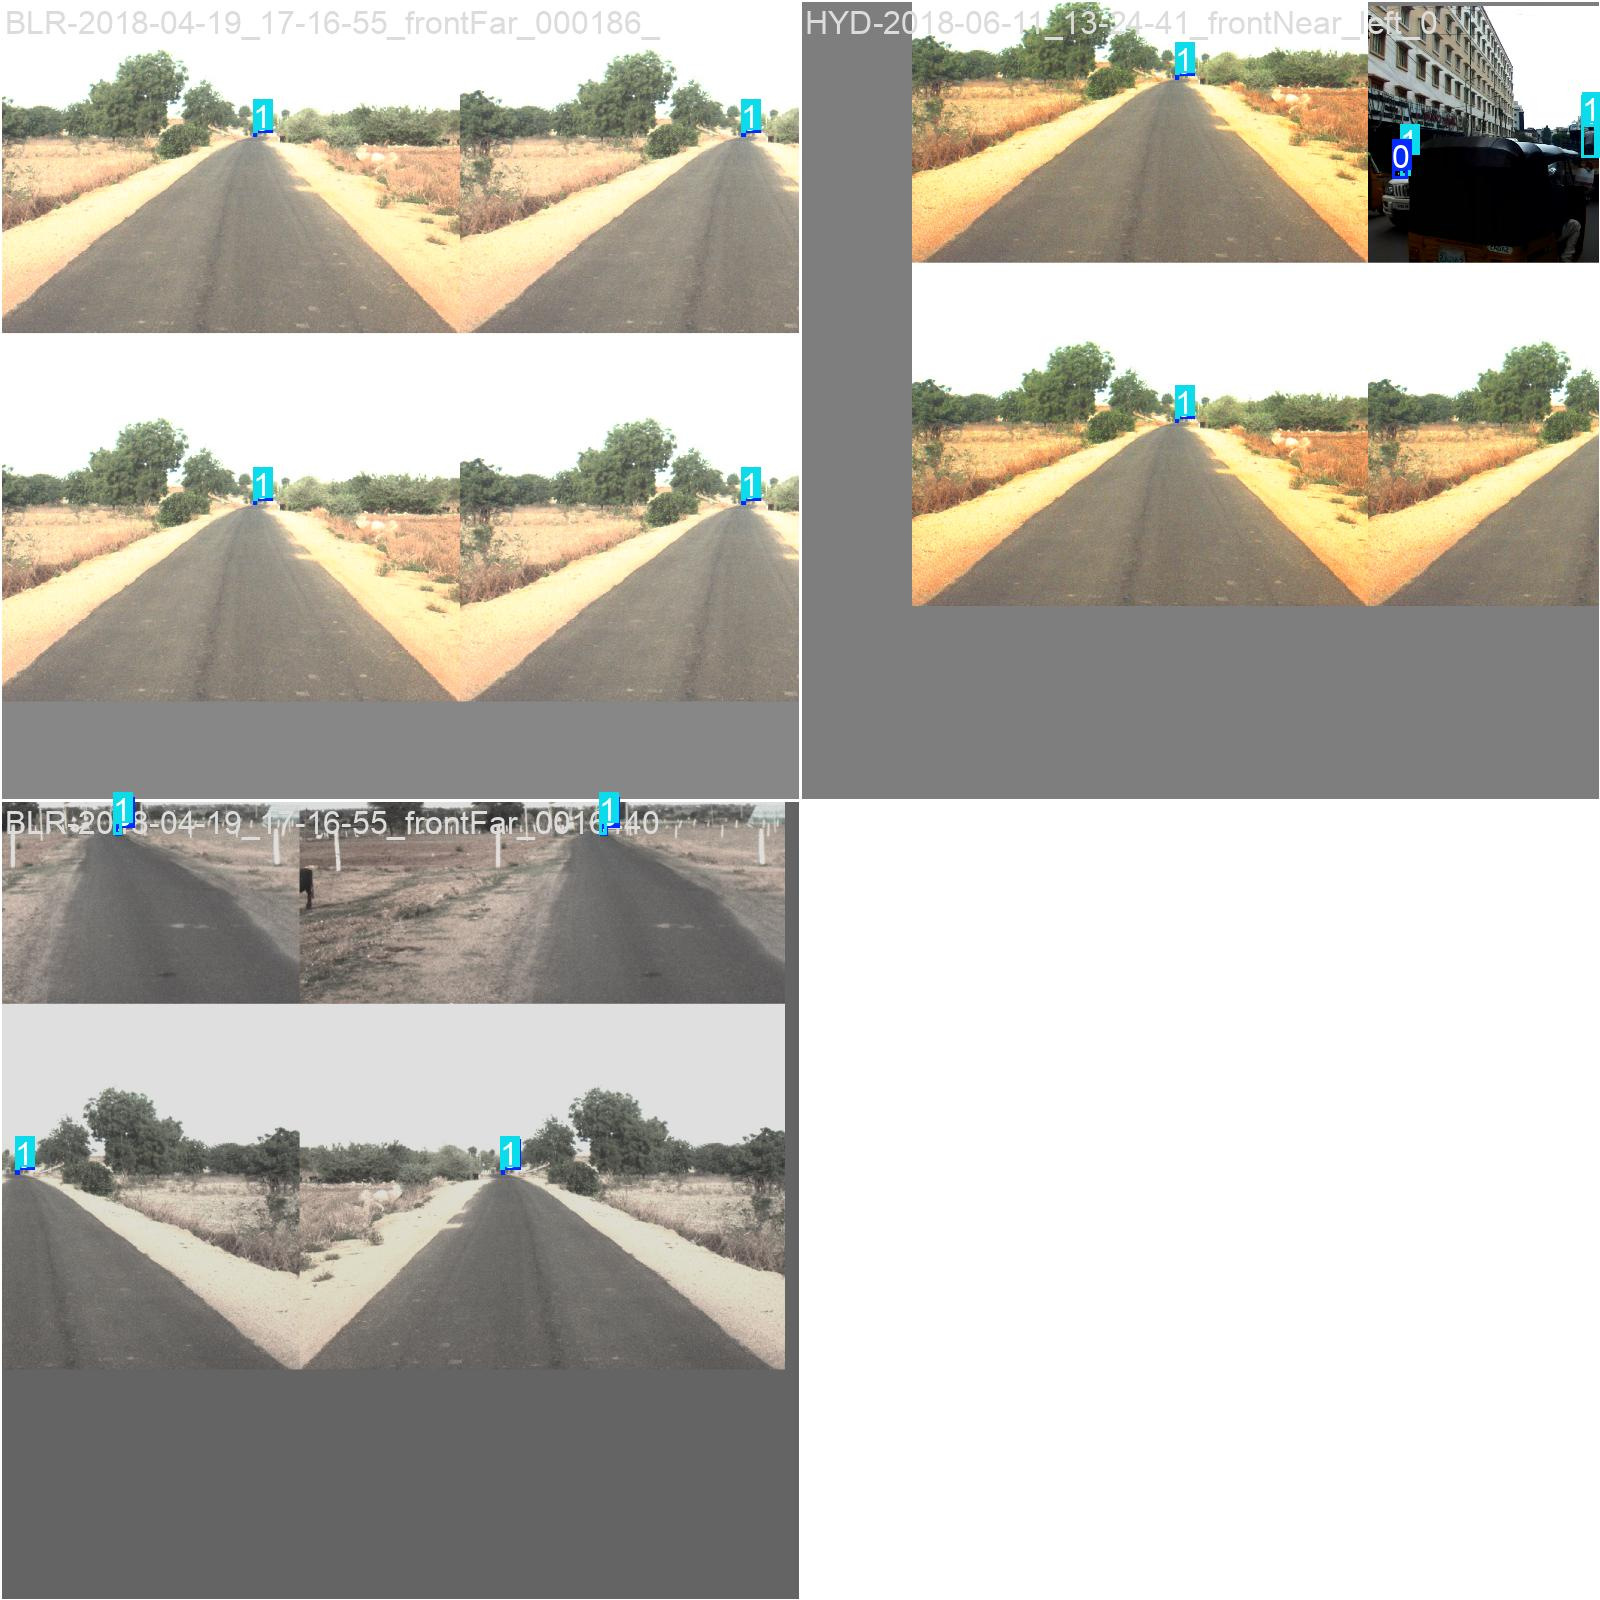
\includegraphics[width=\linewidth]{full_train_batch.jpg}
\caption{Full detector (\texttt{full\_v1-4}, GPU server, 150 epochs)
validation predictions. Blue boxes: \texttt{two\_wheeler};
orange boxes: \texttt{rider}. The model handles both ground-level and
elevated viewpoints drawn from the COCO\,+\,VisDrone corpus.}
\label{fig:full_pred}
\end{figure}

\begin{figure}[H]
\centering
\includegraphics[width=\linewidth, trim=0 0 0 0, clip]%
  {plate_val_pred.jpg}
\caption{Plate detector (\texttt{plate\_v1}, GPU server) validation batch
predictions. Boxes tightly localise \texttt{License Plate} regions across
diverse lighting and angles, confirming mAP50\,=\,0.936 on 150-epoch GPU
training.}
\label{fig:plate_pred}
\end{figure}

\begin{figure}[H]
\centering
\includegraphics[width=\linewidth]%
  {helmet_val_pred.jpg}
\caption{Helmet detector (\texttt{helmet\_v1-2}, GPU server, 200 epochs)
validation predictions. The model correctly discriminates
\texttt{helmet} (green) from \texttt{no\_helmet} (red) in crowded crops
with riders at varying scales.}
\label{fig:helmet_pred}
\end{figure}

\subsection{Confusion Matrices}

Figure~\ref{fig:cms} shows normalized confusion matrices for the plate and
helmet models. The plate detector exhibits near-perfect recall with only
negligible background confusion. The helmet classifier demonstrates strong
separation between the two classes with minimal cross-confusion,
validating the extended 200-epoch training strategy.

\begin{figure}[H]
\centering
\begin{subfigure}[t]{0.48\linewidth}
  \includegraphics[width=\linewidth]%
    {plate_cm.png}
  \caption{Plate detector (\texttt{plate\_v1})}
\end{subfigure}\hfill
\begin{subfigure}[t]{0.48\linewidth}
  \includegraphics[width=\linewidth]%
    {helmet_cm.png}
  \caption{Helmet detector (\texttt{helmet\_v1-2})}
\end{subfigure}
\caption{Normalized confusion matrices. Values represent fraction of
ground-truth samples predicted in each class.}
\label{fig:cms}
\end{figure}

%% ─────────────────────────────────────────────────────────────────────────────
\section{ONNX Inference Optimization}

\subsection{Export and Runtime}

PyTorch weights are exported to ONNX format using Ultralytics' built-in
exporter (\texttt{simplify=True}, opset~17). The export applies operator
fusion, removing training-only gradient nodes and merging adjacent operations
into compound kernels. ONNX Runtime's \texttt{CPUExecutionProvider} uses
multi-threaded OpenMP execution (unavailable in PyTorch eager mode), and
the static computational graph allows ahead-of-time shape inference that
further reduces per-call overhead.

\subsection{Custom Pre/Post-Processing}

The exported ONNX graph produces raw tensors, not parsed result objects.
We implement letterbox preprocessing and coordinate remapping manually:

\textbf{Preprocessing.} The input BGR image is letterbox-resized to
$H_m \times W_m$ (the model's compiled resolution), zero-padded with
value 114 to a square, converted RGB, normalized to $[0, 1]$, and
transposed to \texttt{NCHW} layout as a \texttt{float32} blob.

\textbf{Postprocessing.} The raw output has shape $(1, 4{+}n_c, n_a)$ for
Ultralytics-standard exports---e.g., $(1, 6, 8400)$ for a 2-class model
at 640$\times$640 resolution ($n_a = 8400$ anchor points). Coordinates
are converted from $(c_x, c_y, w, h)$ to $(x_1, y_1, x_2, y_2)$,
de-letterboxed by subtracting pad offsets and dividing by scale, and passed
through greedy Python-side NMS.

\subsection{Production Bug: Inverted Transpose Condition}

\textbf{Symptom.} After deployment, the ONNX backend returned zero detections
on real-world images despite validation mAP50 values of 0.763--0.935.
The PyTorch backend, running the same models, produced correct detections.

\textbf{Diagnosis.} The \texttt{ONNXDetector} determined whether to transpose
the raw output via a \texttt{\_transposed} flag set at load time:
\begin{center}
\small\texttt{\_transposed = (out\_shape[2] > out\_shape[1])}
\end{center}
For the standard Ultralytics output $(1, 6, 8400)$:
$8400 > 6$, so \texttt{\_transposed\,=\,True}.
The postprocessor then executed \texttt{if not \_transposed: pred\,=\,pred.T}---
i.e., it \textit{skipped} the transpose for the very shape that
\textit{required} one. The resulting $(6, 8400)$ tensor was parsed as six
anchor-indexed rows of length 8400 rather than 8400 anchors of length 6,
yielding six meaningless confidence values all below threshold.

\textbf{Fix.} A single condition flip:
\begin{center}
\small\texttt{out\_shape[1] > out\_shape[2]}
\end{center}
This correctly identifies $(1, 8400, 6)$ transposed exports as
\texttt{\_transposed\,=\,True} (no action needed) and $(1, 6, 8400)$
standard exports as \texttt{\_transposed\,=\,False} (transpose
applied). Post-fix, the ONNX backend detected 3 bikes and 3 violations
on a real-world 4-motorcycle image, matching the PyTorch output.

\subsection{Inference Speed}

\begin{figure}[H]
\centering
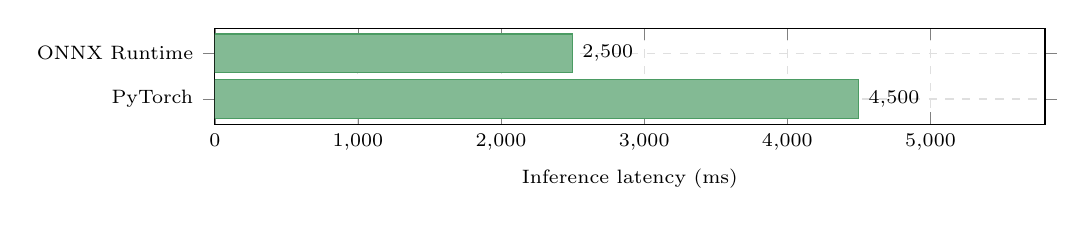
\begin{tikzpicture}
\begin{axis}[
    xbar, width=\linewidth, height=2.8cm,
    bar width=14pt,
    xlabel={Inference latency (ms)},
    symbolic y coords={PyTorch,ONNX Runtime},
    ytick=data,
    xmin=0, xmax=5800,
    xtick={0,1000,2000,3000,4000,5000},
    nodes near coords,
    every node near coord/.append style={font=\scriptsize},
    tick label style={font=\scriptsize},
    label style={font=\scriptsize},
    grid=major, grid style={dashed,gray!25},
    enlarge y limits=0.55,
]
\addplot[fill=successgreen!55, draw=successgreen!80] coordinates {
  (2500,ONNX Runtime) (4500,PyTorch)
};
\end{axis}
\end{tikzpicture}
\caption{End-to-end inference latency on CPU (640$\times$480 JPEG image).
ONNX Runtime achieves \textbf{1.8$\times$} speedup over PyTorch.}
\label{fig:speed}
\end{figure}

Table~\ref{tab:speed} summarizes the performance comparison. The 1.8$\times$
speedup brings the per-image latency below 3~seconds on a mid-range CPU,
making the system viable for real-time checkpoint camera deployments without
dedicated GPU hardware.

\begin{table}[H]
\centering
\small
\caption{Inference latency on CPU (640$\times$480 input).}
\label{tab:speed}
\renewcommand{\arraystretch}{1.15}
\begin{tabular}{lcc}
\toprule
\textbf{Backend} & \textbf{Latency (ms)} & \textbf{Speedup}\\
\midrule
PyTorch (eager mode)  & $\approx$4\,500 & 1.0$\times$\\
ONNX Runtime (CPU EP) & $\approx$2\,500 & \textbf{1.8$\times$}\\
\bottomrule
\end{tabular}
\end{table}

%% ─────────────────────────────────────────────────────────────────────────────
\section{Production API and Frontend}

\subsection{FastAPI Backend}

The \texttt{/predict} endpoint accepts a multipart image upload, validates
the file, offloads inference to a thread pool (keeping the async event loop
free), and returns a structured JSON response. Production hardening:

\begin{itemize}
  \item \textbf{Rate limiting.} Thread-safe token-bucket limiter (20\,req/min
        per IP). Implemented in pure Python using GIL-protected float
        operations---no external dependency on Redis.
  \item \textbf{Input validation.} Four-layer check: file size ($\leq$15\,MB),
        extension whitelist (\texttt{.jpg}, \texttt{.png}, \texttt{.webp},
        \texttt{.bmp}), MIME header advisory, and authoritative magic-bytes
        check via \texttt{imghdr}. Files that pass extension validation but
        fail the magic-bytes check (e.g., renamed executables) are rejected.
  \item \textbf{Async inference.} \texttt{asyncio.run\_in\_executor} offloads
        synchronous ONNX inference to a thread pool. A single Uvicorn worker
        can thus handle concurrent requests without starvation.
  \item \textbf{Structured errors.} All failure modes return consistent
        \texttt{\{"detail": "..."\}} JSON with appropriate HTTP status codes
        (400, 413, 415, 429, 500).
\end{itemize}

\subsection{Web Frontend}

The static frontend is a single-page dark-mode application served directly
by FastAPI. Key UX features include: a drag-and-drop image zone with
file validation feedback; a step-by-step processing tracker
(Upload $\to$ Detect $\to$ Helmets $\to$ Plates); canvas-based animated
bounding-box drawing using \texttt{setLineDash} and
\texttt{requestAnimationFrame}; an inference-time badge populated from the
API response; per-bike violation cards showing rider count, helmet status,
and plate text; and toast notifications for all error conditions.
An \texttt{AbortController} cancels in-flight requests on new image
selection, preventing stale-response rendering.

%% ─────────────────────────────────────────────────────────────────────────────
\section{Deployment Infrastructure}

\subsection{Docker Containerization}

Two Dockerfiles serve different targets:

\textbf{Local (\texttt{Dockerfile}).} Multi-stage build: Stage~1 installs
\texttt{build-essential} and compiles Python wheels; Stage~2 copies only the
compiled wheels into \texttt{python:3.10-slim}, strips compiler toolchains,
compiles source to \texttt{.pyc} bytecode, and switches to a non-root
\texttt{appuser}. The final image exposes port 8000.

\textbf{HF Spaces (\texttt{Dockerfile.hf}).} Inference-only dependencies
(\texttt{requirements\_hf.txt}) reduce the image from $\approx$5\,GB to
$\approx$3\,GB. Port is changed to 7860 (HF Spaces standard). Models are
not baked into the image; instead, \texttt{download\_models.py} fetches the
four ONNX weights (139\,MB total) from a dedicated
\href{https://huggingface.co/hv-123/traffic-sentinel-models}{HF Model Hub
repository} via \texttt{snapshot\_download} at container startup. This
decouples model versioning from application deployment.

\subsection{CI/CD Pipeline}

The GitHub Actions workflow triggers on push to \texttt{main} and on
pull requests. Five jobs run sequentially with dependency gates:
\textbf{lint} (\texttt{ruff} + \texttt{black}),
\textbf{test} (\texttt{pytest -m unit}),
\textbf{docker} (build and push to GitHub Container Registry),
\textbf{compose-test} (\texttt{docker compose up} + \texttt{/api/health} probe),
and \textbf{security} (\texttt{bandit} + \texttt{safety} CVE scan).

%% ─────────────────────────────────────────────────────────────────────────────
\section{Conclusion}

We have presented Traffic Sentinel AI, a production-deployed computer vision
system for two-wheeler traffic violation detection. The cascade architecture
cleanly separates detection, classification, and OCR concerns, allowing
independent dataset curation and architecture selection per sub-task.
ONNX Runtime export delivers a practical 1.8$\times$ CPU speedup enabling
deployment on commodity hardware without GPU infrastructure.

The project spans the full ML engineering lifecycle: dataset engineering
across three public sources, sequential GPU training to overcome memory
constraints, post-deployment ONNX tensor-layout bug diagnosis (a subtle
but critical production issue), API hardening with rate limiting and
magic-bytes validation, modern SaaS frontend development, Docker multi-stage
optimization, and automated CI/CD. The live system is accessible at
\url{https://hv-123-traffic-sentinel-ai.hf.space}.

\textbf{Future directions} include: (i) additional fine-tuning on Indian
traffic imagery to raise the full detector's mAP50 above 0.80; (ii)
integrating the optional YOLOv11-pose model for keypoint-level rider counting;
(iii) TensorRT export targeting $<$500\,ms GPU inference for edge camera
deployments.

%% ─────────────────────────────────────────────────────────────────────────────
\section*{Acknowledgements}
\small
Training infrastructure provided by a dedicated NVIDIA RTX 4060 Ti GPU server.
Datasets sourced from MS COCO 2017, VisDrone 2019, and Roboflow Universe.
The Ultralytics framework was used for all model training and ONNX export.

%% ─────────────────────────────────────────────────────────────────────────────
\begin{thebibliography}{9}
\small
\bibitem{redmon2016yolo}
J. Redmon et al., ``You Only Look Once: Unified, Real-Time Object Detection,''
\textit{CVPR}, pp.\ 779--788, 2016.

\bibitem{wang2024yolov11}
A. Wang et al., ``YOLOv11: An Overview of the Key Architectural Enhancements,''
\textit{arXiv:2410.17725}, 2024.

\bibitem{lin2014coco}
T.-Y. Lin et al., ``Microsoft COCO: Common Objects in Context,''
\textit{ECCV}, pp.\ 740--755, 2014.

\bibitem{zhu2018visdrone}
P. Zhu et al., ``VisDrone-DET2018: The Vision Meets Drone Object Detection
in Image Challenge Results,'' \textit{ECCV Workshops}, 2018.

\bibitem{laroca2018robust}
R. Laroca et al., ``A Robust Real-Time Automatic License Plate Recognition
Based on the YOLO Detector,'' \textit{IJCNN}, 2018.

\bibitem{chen2019helmet}
Y. Chen et al., ``Helmet Use Detection of Tracked Motorcyclists Using
CNN-Based Object Detection,'' \textit{IEEE Access}, vol.\ 7, 2019.

\bibitem{onnx2019}
ONNX Community, ``Open Neural Network Exchange (ONNX),''
\url{https://onnx.ai}, 2019.

\bibitem{jocher2023ultralytics}
G. Jocher et al., ``Ultralytics YOLO,'' \url{https://github.com/ultralytics},
2023.
\end{thebibliography}

\end{document}
